\documentclass[a4paper,ngerman,landscape]{scrartcl}

\usepackage[utf8]{inputenc}

\usepackage[ngerman]{babel}
\usepackage{hyperref}

\usepackage{graphicx}
\usepackage{tikz}
\usetikzlibrary{calc}

\usepackage[protrusion=true,expansion=true]{microtype}

\usepackage{libertine}
\usepackage{tabto}

\setlength\parskip{\medskipamount}
\setlength\parindent{0pt}

\usepackage{geometry}
\geometry{tmargin=0.1cm,bmargin=1.0cm,lmargin=1.5cm,rmargin=1.5cm}

\pagestyle{empty}

\begin{document}

\begin{center}
  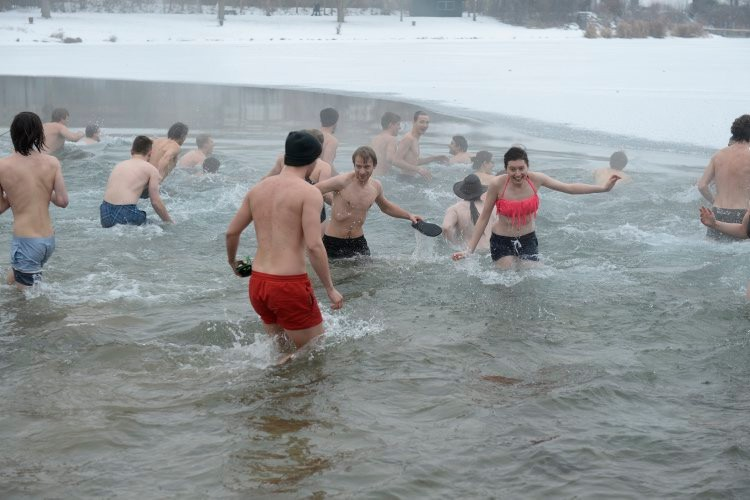
\includegraphics[height=0.15\textwidth]{eisbaden-5}
  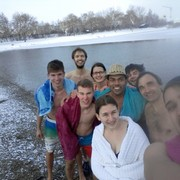
\includegraphics[height=0.15\textwidth]{eisbaden-1}
  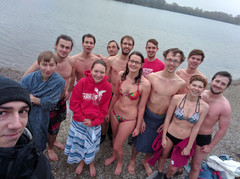
\includegraphics[height=0.15\textwidth]{eisbaden-2}
  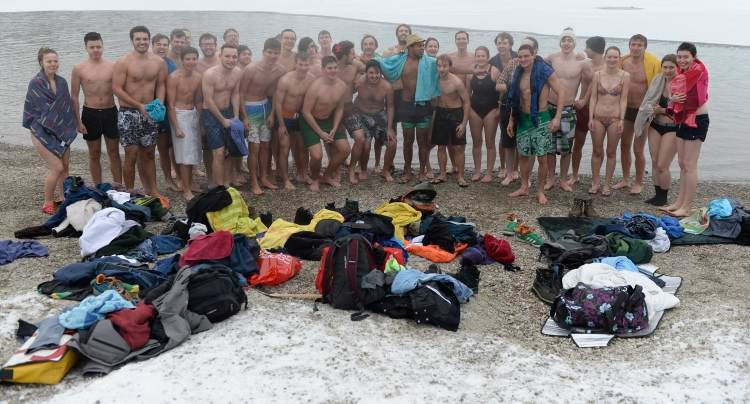
\includegraphics[height=0.15\textwidth]{eisbaden-6}
  \medskip

  \Huge
  \scalebox{3.7}{\textbf{$\!$Mathe-Nachtbaden}}

  \Large
  \begin{minipage}{0.90\textwidth}
    \renewcommand{\baselinestretch}{1.3}

    \setlength\parskip{\medskipamount}
    \vspace{0.3em}
    Im Wintersemester waren wir doch gelegentlich Eisbaden. Jetzt geht's weiter!
    Wir laden alle ein, das \textbf{Nachtbaden am Kuhsee} auszuprobieren.
    Wir treffen uns um 22:23 Uhr beim Restaurant \emph{Seelounge beim Kuhsee}
    und suchen uns dann einen freien Uferabschnitt. Die Zeit ist spät genug,
    damit es schon dunkel ist, und früh genug, damit wir auch zeitig nach Hause
    kommen. Du willst liebend gerne mit, hast aber keine Badesachen in
    Augsburg? Dann musst du nur Merus Lebensmotto beachten:
    \textbf{Jede Hose ist eine Badehose.}

    Wer möchte, kann auf
    {https://etherpad.wikimedia.org/p/nachtbaden-im-mai} nachschauen,
    welche anderen Nacht\-bade\-fans (Studentinnen und Studenten, Mitarbeiterinnen und
    Mitarbeiter, Professorinnen und Professoren) mitgehen, und seinen eigenen
    Namen dazuschreiben.

    \emph{Euer Warmup- und Kreiselteam für verrückte Aktionen :-)}
    \vspace{0.3em}
  \end{minipage}

  \huge
  \scalebox{1.5}{Mittwoch, 31. Mai 2017, 22:23 Uhr beim Kuhsee}

  % http://www.augsburg.de/fileadmin/user_upload/freizeit/baden/fluesse_seen/kuhsee-content-02-zoom.jpg
  \tikz[remember picture,overlay] \node[opacity=1.0,inner sep=0pt] at (current
  page.south){\hspace*{-3cm}\vbox{\vspace*{-4.5cm}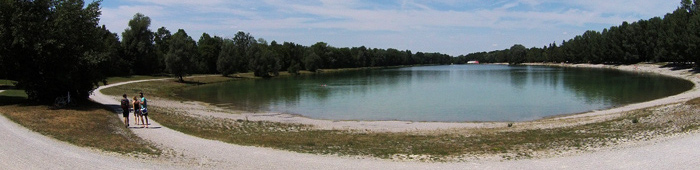
\includegraphics[width=\paperwidth]{kuhsee}}};
\end{center}

\end{document}
